%% This is the ctufit-thesis example file. It is used to produce theses
%% for submission to Czech Technical University, Faculty of Information Technology.
%%
%% Get the newest version from
%% https://gitlab.fit.cvut.cz/theses-templates/FITthesis-LaTeX
%%
%%
%% Copyright 2021, Eliska Sestakova and Ondrej Guth
%%
%% This work may be distributed and/or modified under the
%% conditions of the LaTeX Project Public Licenese, either version 1.3
%% of this license or (at your option) any later version.
%% The latest version of this license is in
%%  https://www.latex-project.org/lppl.txt
%% and version 1.3 or later is part of all distributions of LaTeX
%% version 2005/12/01 or later.
%%
%% This work has the LPPL maintenance status `maintained'.
%%
%% The current maintainer of this work is Ondrej Guth.
%% Contact ondrej.guth@fit.cvut.cz for bug reports.
%% Alternatively, submit bug reports into the tracker at
%% https://gitlab.fit.cvut.cz/theses-templates/FITthesis-LaTeX/issues
%%
%%

% arara: pdflatex
% arara: biber
% arara: pdflatex
% arara: pdflatex

%%%%%%%%%%%%%%%%%%%%%%%%%%%%%%%%%%%%%%%%%
% CLASS OPTIONS
% language: czech/english/slovak
% thesis type: bachelor/master/dissertation
% colour: bw for black&white OR no option for default colour scheme
% electronic or printed: oneside/twoside (default)
%%%%%%%%%%%%%%%%%%%%%%%%%%%%%%%%%%%%%%%%%
\documentclass[english,bachelor,unicode,oneside]{ctufit-thesis}

%%%%%%%%%%%%%%%%%%%%%%%%%%%%%%%%%%
% FILL IN THIS INFORMATION
%%%%%%%%%%%%%%%%%%%%%%%%%%%%%%%%%%
\ctufittitle{Open-source system for cloning RFID/NFC cards and tags} % replace with the title of your thesis
\ctufitauthorfull{Michal Beneš} % replace with your full name (first name(s) and then family name(s) / surname(s)) including academic degrees
\ctufitauthorsurnames{Beneš} % replace with your surname(s) / family name(s)
\ctufitauthorgivennames{Michal} % replace with your first name(s) / given name(s)
\ctufitsupervisor{Ing.\,Jan Fesl,\,Ph.D.} % replace with name of your supervisor/advisor (include academic degrees)
\ctufitdepartment{Department of Information Security} % replace with the department of your defence
\ctufityear{2024} % replace with the year of your defence
\ctufitdeclarationplace{Prague} % replace with the place where you sign the declaration
\ctufitdeclarationdate{\today} % replace with the date of signature of the declaration
\ctufitabstractCZE{Tato práce je zaměřena na problematiku bezpečnosti RFID a NFC tagů a karet v infrastruktuře. Cílem práce je návrh a implementace přenosného a rozšířitelného open-source zařízení, které bude schopné některé vybrané typy RFID karet a tagů klonovat a emulovat za použití vybraného běžně dostupného mikropočítače. Práce je spojena i s vývojem softwaru s grafickým prostředím, který umožňuje potřebné schopnosti zařízení. V teoretické části práce se vysvětlují základní principy fungování technologie RFID, její zabezpečení a nedostatky. Dále probíhá analýza existujících řešení, které se používají pro klonování a emulaci RFID technologií, a výběr vhodného hardwaru pro vytvoření výsledného zařízení. Praktická část práce se zabývá návrhem a samotnou implementací daného zařízení z hardwarové i softwarové stránky. Nakonec je ověřena funkčnost zařízení testováním množinou rozdílných RFID karet a tagů.}
\ctufitabstractENG{This work focuses on the security of RFID and NFC tags and cards in infrastructure. The aim of the work is to design and implement a portable and extensible open-source device that will be able to clone and emulate some selected types of RFID cards and tags using a selected commercially available microcomputer. The work also involves the development of software with a graphical environment that enables the necessary capabilities of the device. The theoretical part of the thesis explains the basic principles of RFID technology, its security and shortcomings. Furthermore, an analysis of existing solutions that are used for cloning and emulation of RFID technology and the selection of suitable hardware for the creation of the resulting device are discussed. The practical part of the thesis deals with the design and actual implementation of the device from both hardware and software aspects. Finally, the functionality of the device is verified by testing a set of different RFID cards and tags.}
\ctufitkeywordsCZE{RFID, NFC, klonování, emulace, bezpečnost informací, Proxmark, Python, Raspberry Pi}
\ctufitkeywordsENG{RFID, NFC, cloning, emulation, information security, Proxmark, Python, Raspberry Pi}
%%%%%%%%%%%%%%%%%%%%%%%%%%%%%%%%%%
% END FILL IN
%%%%%%%%%%%%%%%%%%%%%%%%%%%%%%%%%%

%%%%%%%%%%%%%%%%%%%%%%%%%%%%%%%%%%
% CUSTOMIZATION of this template
% Skip this part or alter it if you know what you are doing.
%%%%%%%%%%%%%%%%%%%%%%%%%%%%%%%%%%

\RequirePackage{iftex}[2020/03/06]
\iftutex % XeLaTeX and LuaLaTeX
    \RequirePackage{ellipsis}[2020/05/22] %ellipsis workaround for XeLaTeX
\else
    \RequirePackage[utf8]{inputenc}[2018/08/11] %this file encoding
    \RequirePackage{lmodern}[2009/10/30] % vector flavor of Computer Modern font
\fi

% hyperlinks
\RequirePackage[pdfpagelayout=TwoPageRight,colorlinks=false,allcolors=decoration,pdfborder={0 0 0.1}]{hyperref}[2020-05-15]

% uncomment the following to hide all hyperlinks
% \RequirePackage[pdfpagelayout=TwoPageRight,hidelinks]{hyperref}[2020-05-15]

\RequirePackage{pdfpages}[2020/01/28]

\setcounter{secnumdepth}{4} % numbering sections; 4: subsubsection



%%%%%%%%%%%%%%%%%%%%%%%%%%%%%%%%%%
% CUSTOMIZATION of this template END
%%%%%%%%%%%%%%%%%%%%%%%%%%%%%%%%%%


%%%%%%%%%%%%%%%%%%%%%%
% DEMO CONTENTS SETTINGS
% You may choose to modify this part.
%%%%%%%%%%%%%%%%%%%%%%
\usepackage{dirtree}
\usepackage{lipsum,tikz}
\usepackage{csquotes}
\usepackage[style=iso-numeric]{biblatex}
\addbibresource{text/bib-database.bib}
\usepackage{listings} % typesetting of sources
% My packages:
\usepackage{tabularx}
\usepackage{fontawesome5}
\usepackage{graphicx}
\usepackage{subcaption}
%\usepackage[newfloat]{minted}\captionsetup[listing]{position=top} % typesetting of sources

%theorems, definitions, etc.
\theoremstyle{plain}
\newtheorem{theorem}{Věta}
\newtheorem{lemma}[theorem]{Tvrzení}
\newtheorem{corollary}[theorem]{Důsledek}
\newtheorem{proposition}[theorem]{Návrh}
\newtheorem{definition}[theorem]{Definice}
\theoremstyle{definition}
\newtheorem{example}[theorem]{Příklad}
\theoremstyle{remark}
\newtheorem{note}[theorem]{Poznámka}
\newtheorem*{note*}{Poznámka}
\newtheorem{remark}[theorem]{Pozorování}
\newtheorem*{remark*}{Pozorování}
\numberwithin{theorem}{chapter}
%theorems, definitions, etc. END
%%%%%%%%%%%%%%%%%%%%%%
% DEMO CONTENTS SETTINGS END
%%%%%%%%%%%%%%%%%%%%%%

\begin{document} 
\frontmatter\frontmatterinit % do not remove these two commands

\includepdf[pages={1}]{benesm41-assignment-en.pdf} % replace that file with your thesis assignment provided by study office

\thispagestyle{empty}\cleardoublepage\maketitle % do not remove these three commands

\imprintpage % do not remove this command

\tableofcontents % do not remove this command
%%%%%%%%%%%%%%%%%%%%%%
% list of other contents: figures, tables, code listings, algorithms, etc.
% add/remove commands accordingly
%%%%%%%%%%%%%%%%%%%%%%
\listoffigures % list of figures
\begingroup
\let\clearpage\relax
\listoftables % list of tables
\lstlistoflistings % list of source code listings generated by the listings package
% \listoflistings % list of source code listings generated by the minted package
\endgroup
%%%%%%%%%%%%%%%%%%%%%%
% list of other contents END
%%%%%%%%%%%%%%%%%%%%%%

%%%%%%%%%%%%%%%%%%%
% ACKNOWLEDGMENT
% FILL IN / MODIFY
% This is a place to thank people for helping you. It is common to thank your supervisor.
%%%%%%%%%%%%%%%%%%%
\begin{acknowledgmentpage}
	I would like to express my highest gratitude to Mr. Jan Fesl for his guidance as my supervisor, to Mr. Tomáš Přeučil for loaning me required hardware and answering my questions, and especially to my family and friends for their support.
\end{acknowledgmentpage} 
%%%%%%%%%%%%%%%%%%%
% ACKNOWLEDGMENT END
%%%%%%%%%%%%%%%%%%%


%%%%%%%%%%%%%%%%%%%
% DECLARATION
% FILL IN / MODIFY
%%%%%%%%%%%%%%%%%%%
% INSTRUCTIONS
% ENG: choose one of approved texts of the declaration. DO NOT CREATE YOUR OWN. Find the approved texts at https://courses.fit.cvut.cz/SFE/download/index.html#_documents (document Declaration for FT in English)
% CZE/SLO: Vyberte jedno z fakultou schvalenych prohlaseni. NEVKLADEJTE VLASTNI TEXT. Schvalena prohlaseni najdete zde: https://courses.fit.cvut.cz/SZZ/dokumenty/index.html#_dokumenty (prohlášení do ZP)
\begin{declarationpage}
I hereby declare that the presented thesis is my own work and that I have cited all sources of
information in accordance with the Guideline for adhering to ethical principles when elaborating an
academic final thesis.
I acknowledge that my thesis is subject to the rights and obligations stipulated by the Act No.
121/2000 Coll., the Copyright Act, as amended, in particular the fact that the Czech Technical
University in Prague has the right to conclude a licence agreement on the utilization of this thesis as
a school work pursuant of Section 60 (1) of the Act.
\end{declarationpage}
%%%%%%%%%%%%%%%%%%%
% DECLARATION END
%%%%%%%%%%%%%%%%%%%

\printabstractpage % do not remove this command


%%%%%%%%%%%%%%%%%%%
% ABBREVIATIONS
% FILL IN / MODIFY
% OR REMOVE ENTIRELY
% List the abbreviations in lexicography order.
%%%%%%%%%%%%%%%%%%%
\chapter{List of abbreviations}
	
\begin{tabular}{rl}
BS & Base-Station\\
GUI & Graphical User Interface\\
HF & High Frequency\\
LF & Low Frequency\\
NFC & Near Field Communication\\
UID & Unique Identifier\\
UI & User Interface\\
RFID & Radio Frequency Identification\\
\end{tabular}
%%%%%%%%%%%%%%%%%%%
% ABBREVIATIONS END
%%%%%%%%%%%%%%%%%%%

\mainmatter\mainmatterinit % do not remove these two commands

%%%%%%%%%%%%%%%%%%%
% THE THESIS
% MODIFY ANYTHING BELOW THIS LINE
%%%%%%%%%%%%%%%%%%%


%---------------------------------------------------------------
\setcounter{page}{1}

% Do not forget to include Introduction
%---------------------------------------------------------------
% \chapter{Introduction}
% uncomment the following line to create an unnumbered chapter
\chapter*{Introduction}\addcontentsline{toc}{chapter}{Introduction}\markboth{Introduction}{Introduction}
%---------------------------------------------------------------
\setcounter{page}{1}

% The following environment can be used as a mini-introduction for a chapter. Use that any way it pleases you (or comment it out). It can contain, for instance, a summary of the chapter. Or, there can be a quotation.
% \begin{chapterabstract}
% 	\lipsum[1]
% \end{chapterabstract}

Nowadays, the importance of RFID and NFC technologies has become increasingly crucial. People come across these technologies daily, validating their tickets in public transportation, accessing their offices, and paying with a card in a store. However, their significance extends beyond these everyday applications.

For instance, this innovation revolutionized the way businesses operate and interact with their environments. In retail, RFID tags have brought improvements in commodity management, allowing retailers to have a perfect overview of the stock levels in real time and optimize the supply to maximum efficiency. Logistic management benefits from RFID's ability to track the goods throughout the whole distribution process, reducing delays and eliminating certain management errors. In healthcare, NFC devices help with patient identification and medication administration, improving safety, accuracy, and the speed of healthcare processes. \cite{pirrone2012mobile} Similarly, the NFC technology is used in public transportation for ticketing, offering commuters a smart and convenient methods of payment and entry.

The history of RFID/NFC technologies can be traced back to World War II. The air forces of several countries were using radar, which was discovered in 1935 by physicist Sir Robert Alexander Watson-Watt, to warn of approaching airplanes. Germans discovered a method of identifying an enemy aircraft from allied aircraft by scanning the difference in the radio signal reflected by the airplane when the airplane rolled. This could be considered one of the earliest instances of passive RFID system in history. Later on, Sir Watson-Watt came up with the first active system, the so-called "identification friend or foe" system. Brits put an active transmitter on each airplane and when it received signals from the radars on the ground, it started broadcasting a signal back, identifying the airplane as friendly. Over the decades, significant advancements appeared. The first official active rewritable RFID tag was introduced in the 1970s by Mario W. Cardullo. That same year, Charles Walton received a patent for a passive transponder used to unlock doors. U.S. government had also an enormous influence on the development of this technology. Scientists from the Los Alamos National Laboratory developed a system to track nuclear materials in the area. Later, at the request of the Agricultural Department, Los Alamos also developed a system to track cows. Every cow has to be given hormones and medicines when it is ill and it was really hard to keep track of cows so that they do not receive two doses accidentally.~\cite{violino2005history}

As time went on, RFID and NFC technologies started to be used in more and more industries, as people realized the benefits it provides. These technologies continue to evolve rapidly, driven by innovations such as extended read ranges or enhanced data encryption. The adoption of NFC in smartphones has even further accelerated the integration into everyday life, enabling for example contactless payments or data transfer.

Many security systems heavily rely on RFID/NFC technologies for access control, authentication, or asset protection. The access systems that are commonly found in office buildings, hotels, or even houses, use this technology to grant or restrict entry based on authorized credentials. Asset tracking solutions use tags to monitor the location or movement of valuable assets, reducing the risk of a theft.

% Motivation
My motivation to pursue this topic was driven by my interest in the subject of RFID access control and identification, which was invoked by popular cloning device solutions such as Flipper Zero and the discussions that arose around these technologies. The creation of the resulting device would help to add to my surface understanding of the subject and the field, which is increasingly utilized nowadays and whose security must be appealed to.

% Importance
The outcome of this work should help readers to understand the basic principles of the RFID technology, with practical application enabled through the created device. Additionally, this study seeks to uncover security flaws in this particular technology sector, where some of them can be effortlessly exploited by the resulting device.

% Focus of the thesis
In this thesis, I undertake a detailed analysis of existing hardware used for RFID/NFC tag reading, cloning, or emulating, which is available on the market and could be used for the resulting open-source cloning device. Later on, I also address the actual design of the architecture of such a device, along with the design of the software enabling cloning or emulation. This software includes a user interface allowing simple interaction and use of its features. Furthermore, I provide the implementation process of the software, including the steps taken to ensure hassle-free integration with the used hardware components. Finally, I test the developed device with different types of tags and evaluate its functionality and reliability.

\chapter{Goals}
\label{chap:goals}

The main goal of this thesis is to deal with a development of a portable open-source device, that will be able to clone and emulate RFID/NFC tags of various types. More precisely, the following sub-tasks are set:

\begin{itemize}

    \item \textbf{Hardware and software architecture design} --- design a hardware and software architecture of an open-source device with regard to modularity and future expandability. The device must function as a stand-alone unit without the need to connect to a personal computer. To implement the device, use one of the commonly available microcomputers such as Raspberry Pi, Arduino or similar.

    \item \textbf{Software development} --- create software in C++ or Python programming language that allows cloning and emulation of RFID/NFC card/tags of at least 3 different types such as Mifare Classis, Mifare Ultralight, Mifare Desfire v1 etc. Debug the software directly in the environment of the selected microcomputer.

    \item \textbf{User interface implementation} --- implement a user interface to control the device that allows the user to easily interact with the device and use its features.

    \item \textbf{Testing} --- test the finished device on different types of RFID/NFC cards/tags and evaluate its functionality.

\end{itemize}
\chapter{Theoretical background}
\label{chap:theory}

This chapter provide all the important information to understand the problematics of RFID systems.

\chapter{Analysis}
\label{chap:analysis}

This chapter presents an analysis of the existing hardware. It outlines the capabilities of existing RFID/NFC readers, cloners, emulators, microcomputers, and other relevant hardware components. Specifically focusing on readers, it compares the devices based on various parameters, including compatibility with certain tag types, limitations, and pricing. Additionally, other hardware components are evaluated based on their capabilities and compatibility with RFID readers. The objective is to determine the most suitable device for integration into the portable device developed in this thesis, meeting the specified requirements effectively.


\section{Requirements}
\label{sec:requirements}

This section sets the requirements for the components of the resulting device. It describes the desired characteristics of the RFID/NFC reader, microcomputer, and its components. The resulting device composed of individual components should meet the goals specified in Chapter~\ref{chap:goals}.

\subsection{RFID/NFC Reader Requirements}

As written in Chapter~\ref{chap:theory}, there are types of tags that are easy to clone or emulate, as their main aim is to provide availability rather than integrity or confidentiality of data. In other words, some types of tags do not prioritize providing security measures. For instance, a simple 125 kHz EM410x tag holds data that can be easily read without any constraints and can be cloned or emulated quite effortlessly. Certain tags are designed to provide users with security but have failed in secure implementation. For example, their encryption algorithm has been reverse-engineered, and a variety of attacks have been published, effectively compromising their security\footnote{A perfect example of such tags are those using the encryption algorithm Crypto-1}. These tags are a little more complicated to clone, as some type of attack must be executed against the tag, exploiting its vulnerabilities. Lastly, there are tags for which no vulnerabilities or published attacks are known.

It would be beneficial to utilize an open-source reader capable of reading, writing, emulating tags, and exploiting the known vulnerabilities of some of the tags all by itself. This would help to narrow the scope of the thesis, as otherwise, the work would be very extensive. Also, the reader must be operable from the external microcomputer.

\subsection{Microcomputer Requirements}

There are various requirements for the microcomputer. One of the most crucial aspects when searching for a suitable microcomputer is its ability to communicate with the chosen reader effectively. The communication should be implementable using the chosen programming language, with minimal limitations. Another critical parameter is the ability to control the microcomputer. Most certainly, there should be a way to connect a small screen to the device. The device should be controlled via a touchscreen or connected buttons. The power consumption of the microcomputer must also be taken into account to ensure that the resulting portable device is capable of lasting a satisfying period of time.


\subsection{User Interface Requirements}

The UI of the device should meet several properties. The main characteristic may be considered the simplicity --- the device should be easy to use without any extra thinking. Another important property is the ability to enter characters. However, this, in a way, restricts the usage of physical buttons because there would have to be either too many buttons, or the entering of the characters would be too slow. This determines the direction to use a touch display instead. This way, the UI would be simple and user-friendly, without many limitations. 

The power consumption of the display is also an important evaluation criterion, and so is the size of the display, which should not be too big.


\section{Existing RFID/NFC Cloners}

This section covers various existing solutions, and devices capable of cloning or emulating tags. It provides a general overview of their capabilities, prices, and potential limitations.

\subsection{Flipper Zero}

The Flipper Zero is one of the most well-known gadgets. Among its capabilities, such as emulating a BadUSB device\footnote{A so-called BadUSB device is a device that is recognized by computers as a human interface device, such as a keyboard~\cite{badusb}.} or controlling devices that utilize radio signals below 1 GHz, it can also operate at frequencies of 125 kHz and 13.56 MHz for RFID tags~\cite{flipper}. It offers a highly portable solution for reading, writing, cloning, and emulating tags, supporting various types, such as MIFARE Classic 1k or MIFARE Ultralight~\cite{flipperreading}.  Its software is licensed under GPL-3.0, making it fully modifiable and distributable under the same license~\cite{githubflipper}.

The device is powered by an integrated lithium-ion polymer rechargeable battery, with power management efficiently handled to provide operation for up to a month without recharging.~\cite{flipperpower}

However, a significant drawback is the fact that this device is already a completely standalone unit. The device is available for purchase on the official website for 165 Euros~\cite{flippershop}. Although this price may seem high, it is essential to consider that the device offers significantly more functionalities than those outlined in Section~\ref{sec:requirements}.


\subsection{Chameleon Mini}

The Chameleon Mini is a versatile credit-card shaped RFID and NFC tool, often used for security compliance, analysis, penetration testing, and various applications. Its fully open-source platform supports emulating perfect clones of various commercial smartcards, including the UID and even cryptographic functions. Its human-readable command set provides users the ability to configure settings and content for up to 8 internally stored virtual cards. Integrated buttons and LEDs enable user interaction while in standalone mode, meaning when the device is not connected to the computer.~\cite{chameleonwiki}

Despite its capability to read and emulate various types of high frequency cards, its firmware does not provide the ability to write cards. To crack cards, the device itself supports only a MFKey32 attack, where the attacker has to have also an access to the reader itself to catch and decode transmitted keys. This does not quite meet our requirements. ~\cite{lab401chameleon}

Its battery life is quite extensive, it contains a Li-ion battery which is capable of running the device for up to 1 year with an average usage of 15 seconds a day. The device is quite expensive, it can be purchased for around 130 Euros.~\cite{lab401chameleon}

This powerful and highly modifiable device supports the emulation of cards of various types, however, its software cannot write cards.


\subsection{Chameleon Ultra}

Chameleon Ultra is a relative of Chameleon Mini, one of the smallest solutions in existence. It's about the size of a keychain, capable of reading, emulating, writing, and even cracking tags. It boasts better emulation capabilities than Flipper Zero, but also than Proxmark.~\cite{chameleonultra}

It is controlled via CLI and GUI interfaces, but can also be controlled via a mobile app. Includes a 90 mAh LiPo battery that lasts up to a month without a charge.~\cite{chameleonultra}

Its huge disadvantage is its price. The device is available for 155 euros~\cite{chameleonultra}. The huge advantage is its capabilities in comparison, if we think about the size of the device.

This device meets all the requirements, but the decision must take into account its price. 


\subsection{NXP PN532 Module}

The NXP PN532 is a highly integrated module operating at 13.56 MHz frequencies. It supports 6 different operating modes,
\begin{itemize}
    \item ISO/IEC 14443A/MIFARE Reader/Writer,
    \item FeliCa Reader/Writer,
    \item ISO/IEC 14443B Reader/Writer,
    \item ISO/IEC 14443A/MIFARE Card MIFARE Classic 1K or MIFARE Classic 4K card emulation mode,
    \item FeliCa Card emulation, and
    \item ISO/IEC 18092, ECMA 340 Peer-to-Peer.~\cite{pn532doc}
\end{itemize}

With various libraries, it is possible to perform for example an offline nested attack~\cite{nestedpn532} or a darkside attack~\cite{darksidepn532} in the computer. However, these attacks are not done in the module itself, but in the connected computer.

Another library makes possible to write Gen 3 Magic MIFARE Classic tags and Gen 2 Magic MIFARE Classic tags.~\cite{clonerpn532}

It can be classified as an affordable device, a man can buy this device for only around 10 Euros.~\cite{pn532shop}

This device can be controlled via Arduino microcontroller, however, its downside is the restriction to 13.56 MHz frequencies.


\subsection{Proxmark}

The Proxmark is an RFID tool, supporting vast majority of RFID tags worldwide. It allows both low level and high level interactions with the tags. It is adapted to many industries and users, its possibilities are used by people from the academic research, product development or penetration testing.~\cite{proxmark}

Its functionalities include the ability to read tags, write tags, write magic tags, simulate tags, and even crack the tags, meaning the Proxmark software includes attacks against various known tags vulnerabilities. \cite{proxmarkwiki}

There are a number of variants of the Proxmark on the market, including cheap clones, which however can be flashed with the software and are supported.~\cite{proxmarkclones}

The device can be connected to a computer with an USB cable and it is controlled via a command-line interface~\cite{proxmarkcommands}. It also supports a standalone mode, which is a mode, in which the device can be utilized without connection to the computer. However, the standalone mode is quite limiting, because the device itself contains only one simple button and LED indicators - this does not allow more complicated user input.~\cite{proxmarkstandalone}

The price of one of the cheaper variants of the Proxmark, the Proxmark 3 Easy, is around 75 Euros~\cite{proxmarkshop}.


\section{Existing Microcomputers}

This section covers various existing microcomputers. Provides a general overview of the capabilities, and options for connecting other modules, such as displays or the reader itself.


\subsection{Arduino}

Arduino is an open-source platform featuring easy to use hardware boards, containing a microcontroller, and input/output pins for connecting all kinds of peripherals. It is programmable by \emph{Arduino programming language}, which is based on \emph{Wiring}\footnote{\emph{Wiring} is an open-source programming framework for microcontrollers~\cite{wiring}.}.~\cite{arduino}

There are available many types of Arduino boards, that vary in size, number of pins or computing power.~\cite{arduinohardware} Also, there are available many Arduino accessories, including various types of screens, buttons, or even RFID/NFC readers\footnote{As an example could be used the aforementioned PN532 module.}. 

It is still safe to say that the price of the boards is quite low, even more when Arduino clones\footnote{These clones are cheaper unofficial versions of the original Arduino boards.} are taken to consideration.


\subsection{Raspberry Pi}

Raspberry Pi produces a series of single-board modular microcomputers that are built on the Arm architecture and also Raspberry Pi Pico boards for lower-power and real-time applications. The series of microcomputers run the Linux operating system, which makes them exceptionally potent for a diverse number of tasks. Every Raspberry Pi board is backed by extensive technical documentation, and enthusiastic community.~\cite{raspberry}

Each board has several input/output pins, number of models contain also RJ45 network ports, USB ports, or even HDMI ports.

Similar to the Arduino, the Raspberry Pi has many modules available, including screens, for which there are open-source drivers and libraries available.

The price of a Raspberry Pi 4 model B, containing all the ports mentioned previously, goes from 35 Euros~\cite{raspberryshop}.


\section{Comparison}

For clarity, following tables give an overview of the properties of all components. This will help to select the most suitable ones.

\subsection{Comparison of Readers}

\begin{table}[h]
    \caption[Readers comparison]{~Comparison of tag readers}\label{tab:readers}
    \centering
    \renewcommand{\arraystretch}{1.3}
    \begin{tabularx}{\textwidth}{@{}l *7{|>{\centering\arraybackslash}X}}
    Device &  LF & HF & Read & Crack & Write magic & Emulate & Price \\ \hline \hline
    Flipper Zero & \faCheck & \faCheck & \faCheck & \faCheck & \faCheck & \faCheck & High \\ \hline
    ChameleonMini & ~ & \faCheck & \faCheck & ~ & ~ & \faCheck & High \\ \hline
    ChameleonUltra & \faCheck & \faCheck & \faCheck & \faCheck & \faCheck & \faCheck & High \\ \hline
    PN532 module & ~ & \faCheck & \faCheck & ~ & \faCheck & \faCheck & Low \\ \hline
    Proxmark & \faCheck & \faCheck & \faCheck & \faCheck & \faCheck & \faCheck & Middle \\ 
    \end{tabularx}
\end{table}

The Table~\ref{tab:readers} shows a comparison of the mentioned RFID/NFC tag readers. Only Proxmark and Chameleon Ultra meet the specified requirements, as the other readers mentioned lack important features, such as low-frequency card support for the NIX PN532 module and Chameleon Mini. The Flipper Zero does not meet our requirements as it is already a standalone unit --- the Flipper Zero could not be used as a component in the final device.

The Chameleon Ultra ticks all the boxes, but is very expensive for the purposes of this thesis. In contrast, the price of Proxmark is satisfactory because it is far from the highest and still meets all the conditions.

The big advantage of Proxmark is a great support --- the Github repository containing the device firmware and also the desktop client is regularly updated. A disadvantage may be the size of the device, the Proxmark 3 Easy type has dimensions of 54 mm × 86.6 mm~\cite{dimensionsproxmark}. However, this might not matter so much, it will also depend on the size of the microcomputer selected. 

Since the Proxmark is the most capable of the devices analyzed and the price is acceptable, this device is chosen as the reader used for this project.


\subsection{Comparison of Microcomputers}

\begin{table}[h]
    \caption[Microcomputers comparison]{~Comparison of microcomputers}\label{tab:microcomputers}
    \centering
    \renewcommand{\arraystretch}{1.3}
    \begin{tabularx}{\textwidth}{@{}l *5{|>{\centering\arraybackslash}X}}
    Device &  Easy communication with Proxmark & Energy consumption & Touch display available & Capabilities & Price \\ \hline \hline
    Arduino & ~ & Low~\cite{arduinodoc} & \faCheck & Low & Low \\ \hline
    Raspberry Pi & \faCheck & High~\cite{raspberrydoc} & \faCheck & High & Low \\
    
    \end{tabularx}
\end{table}

The Table~\ref{tab:microcomputers} shows a comparison of the mentioned microcomputers. Both options are strong candidates, but implementing Arduino communication with Proxmark would be much more challenging than providing Raspberry Pi communication via USB port. 

In terms of extensibility, again, both are very good, but the Raspberry Pi is slightly better. With the computational power of the Raspberry Pi, other types of attacks could be implemented in the future, with the computations taking place within the microcomputer itself. The Raspberry itself has Bluetooth and Wi-Fi support built in by default, and in the future it would be much easier to control the device via, for example, a mobile phone than it would be with an Arduino.

Likewise, implementing a software user interface will be much easier on the Raspberry Pi, as it runs Linux and thus has many graphical programming language libraries to choose from.  

The disadvantages of the Raspberry Pi may be its size and power consumption, which is high compared to the Arduino. 


\section{Conclusion of the Analysis}

Several RFID/NFC reader solutions were analysed, and it was found that many of them could function as standalone units. After careful consideration of the requirements, Proxmark was selected as the most suitable reader for our project. Additionally, the Raspberry Pi was identified as the most appropriate microcomputer for this work.

After analyzing the different types of Proxmark, the Proxmark 3 Easy was selected. It is one of the cheapest variants of Proxmark and at the same time it is not deprived of any important functionality.

After analyzing the different types of Raspberry Pi, the Raspberry Pi 4 B variant with 4 GB of RAM was selected. This variant is one of the newer and more powerful ones. However, it is also quite large, but this does not matter because the selected Proxmark 3 Easy is almost the same size and therefore choosing a smaller microcomputer would not reduce the overall size of the resulting device.

The Waveshare 3.5" LCD touchscreen is suitable as a display for the device, which is the same size as the Raspberry Pi and Proxmark. It is connected and powered via 26 pins. There are freely available drivers to make it easily usable.~\cite{waveshare35inch}

\begin{figure}[h]
    \centering
    \begin{minipage}[b]{0.45\textwidth}
        \centering
        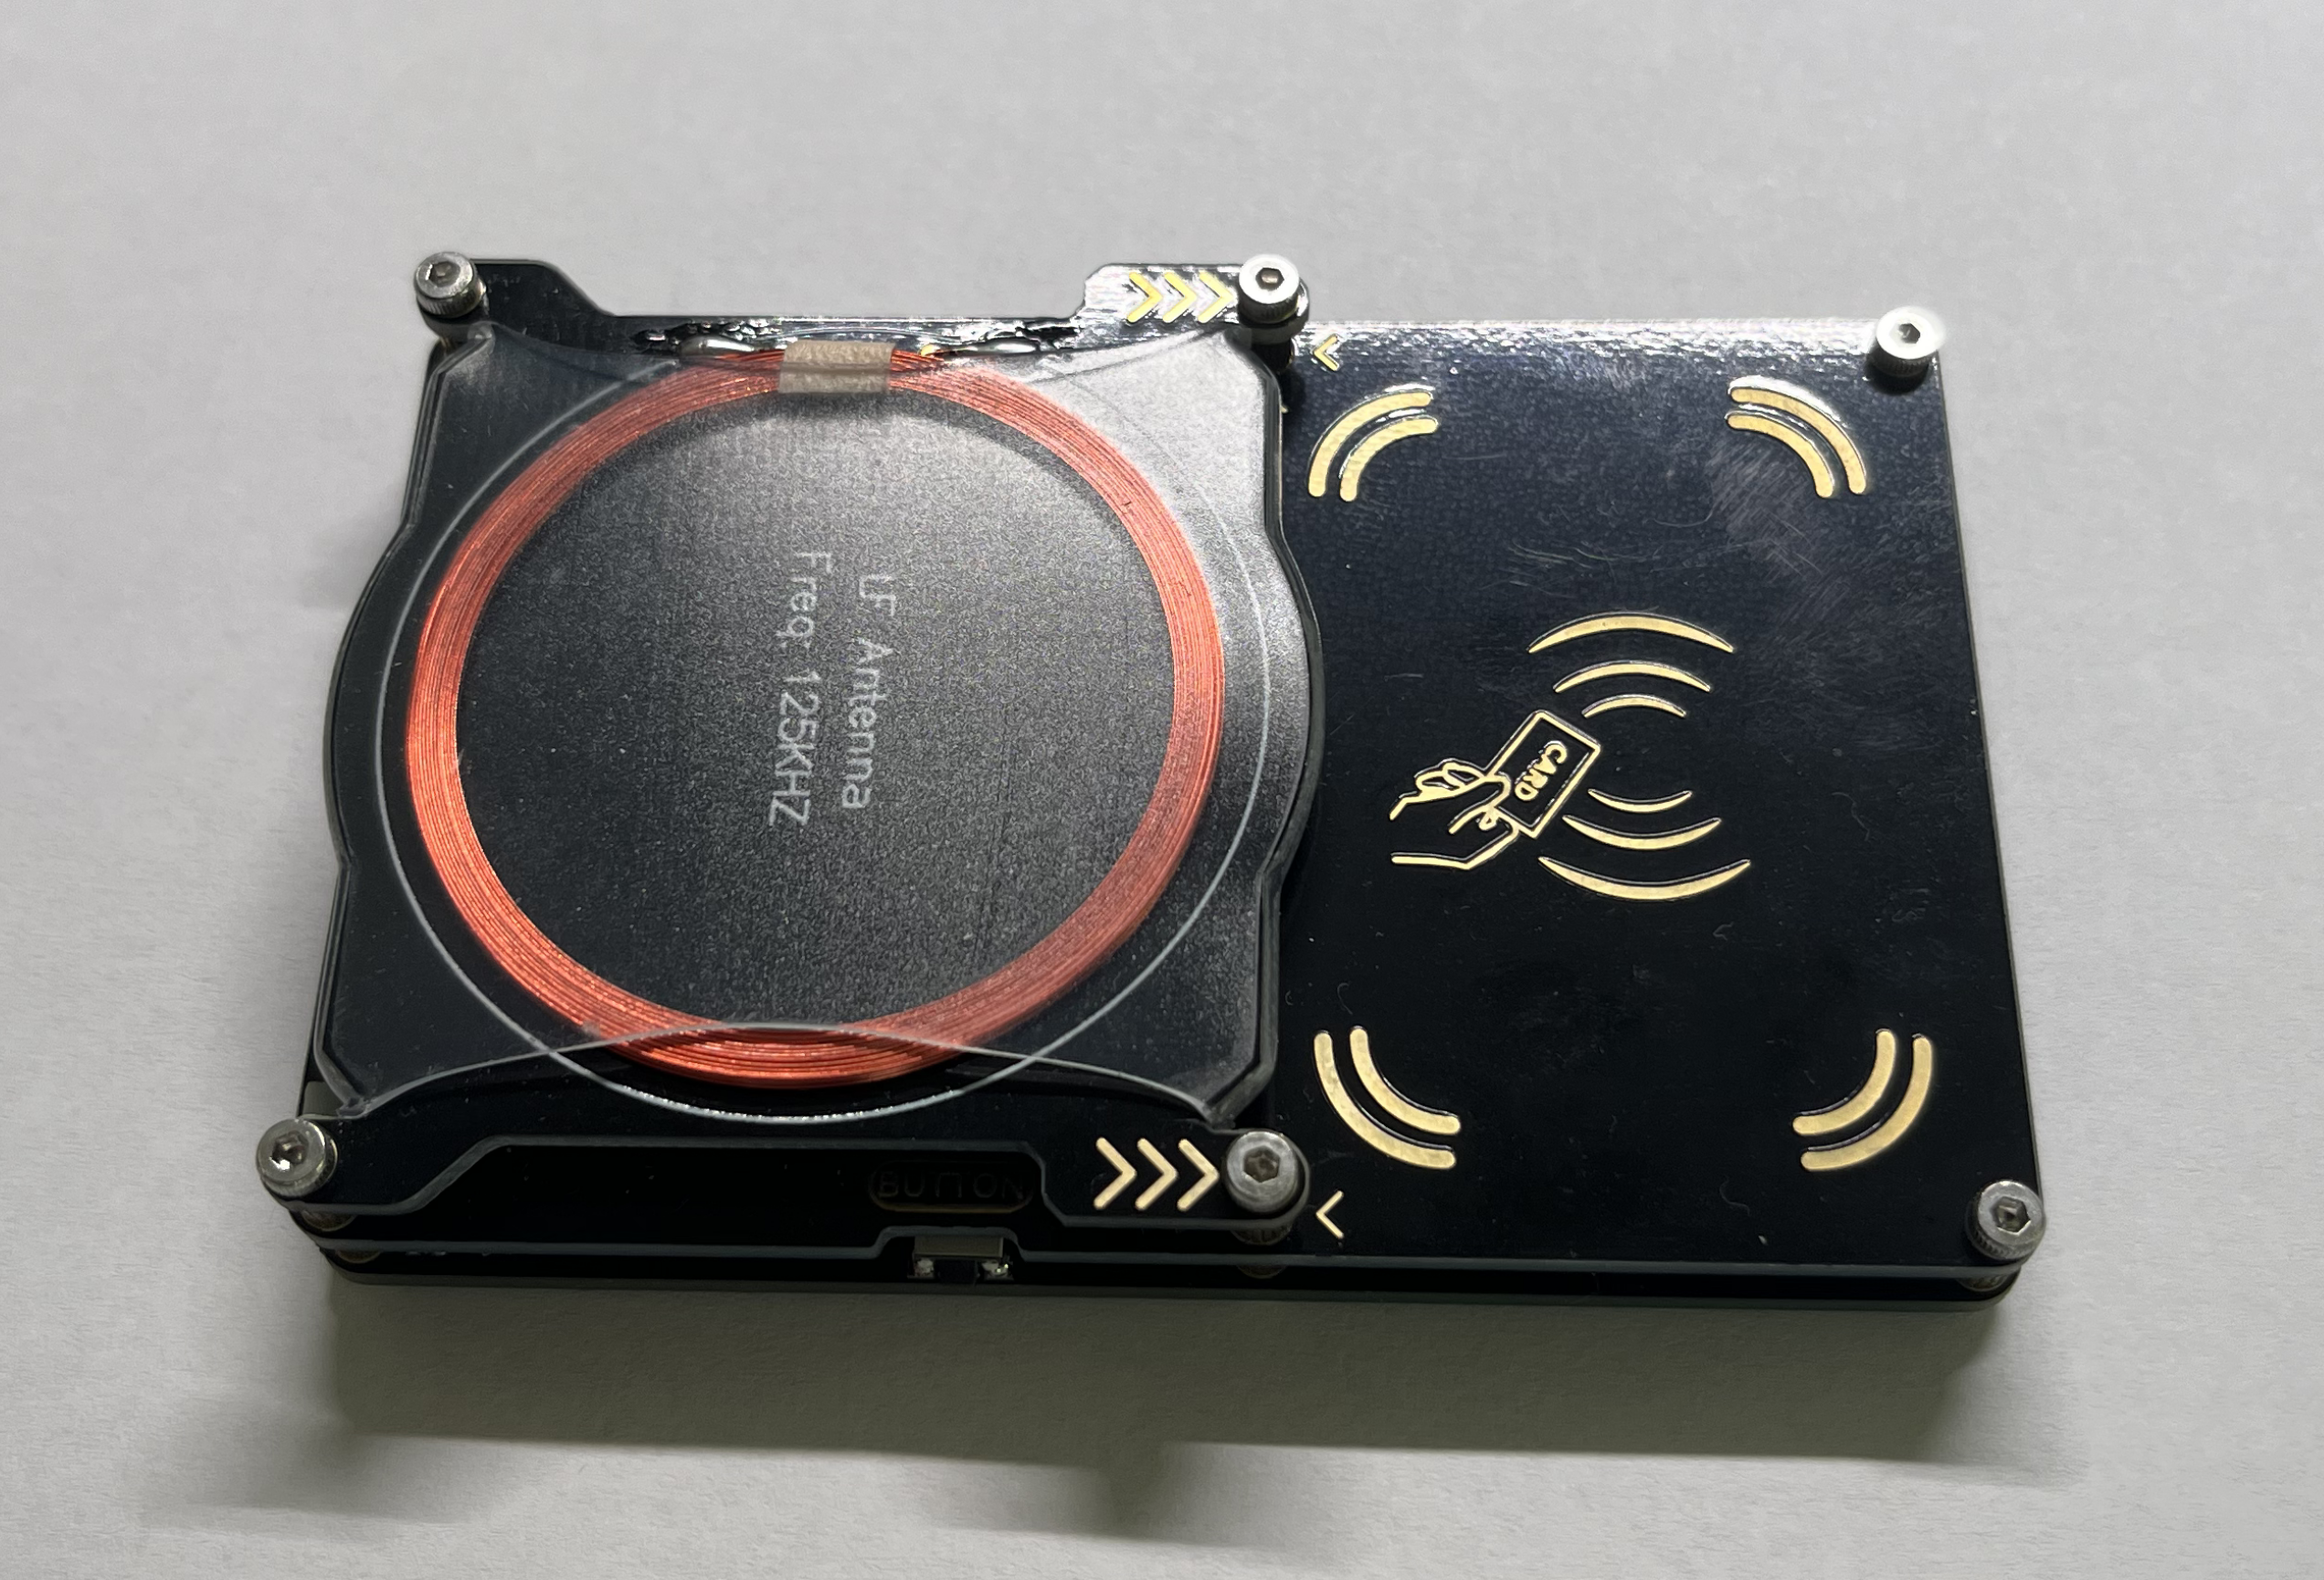
\includegraphics[width=\textwidth]{text/proxmark.png}
        \caption{~Photo of Proxmark 3 Easy}
        \label{fig:sub1}
    \end{minipage}
    \hfill
    \begin{minipage}[b]{0.45\textwidth}
        \centering
        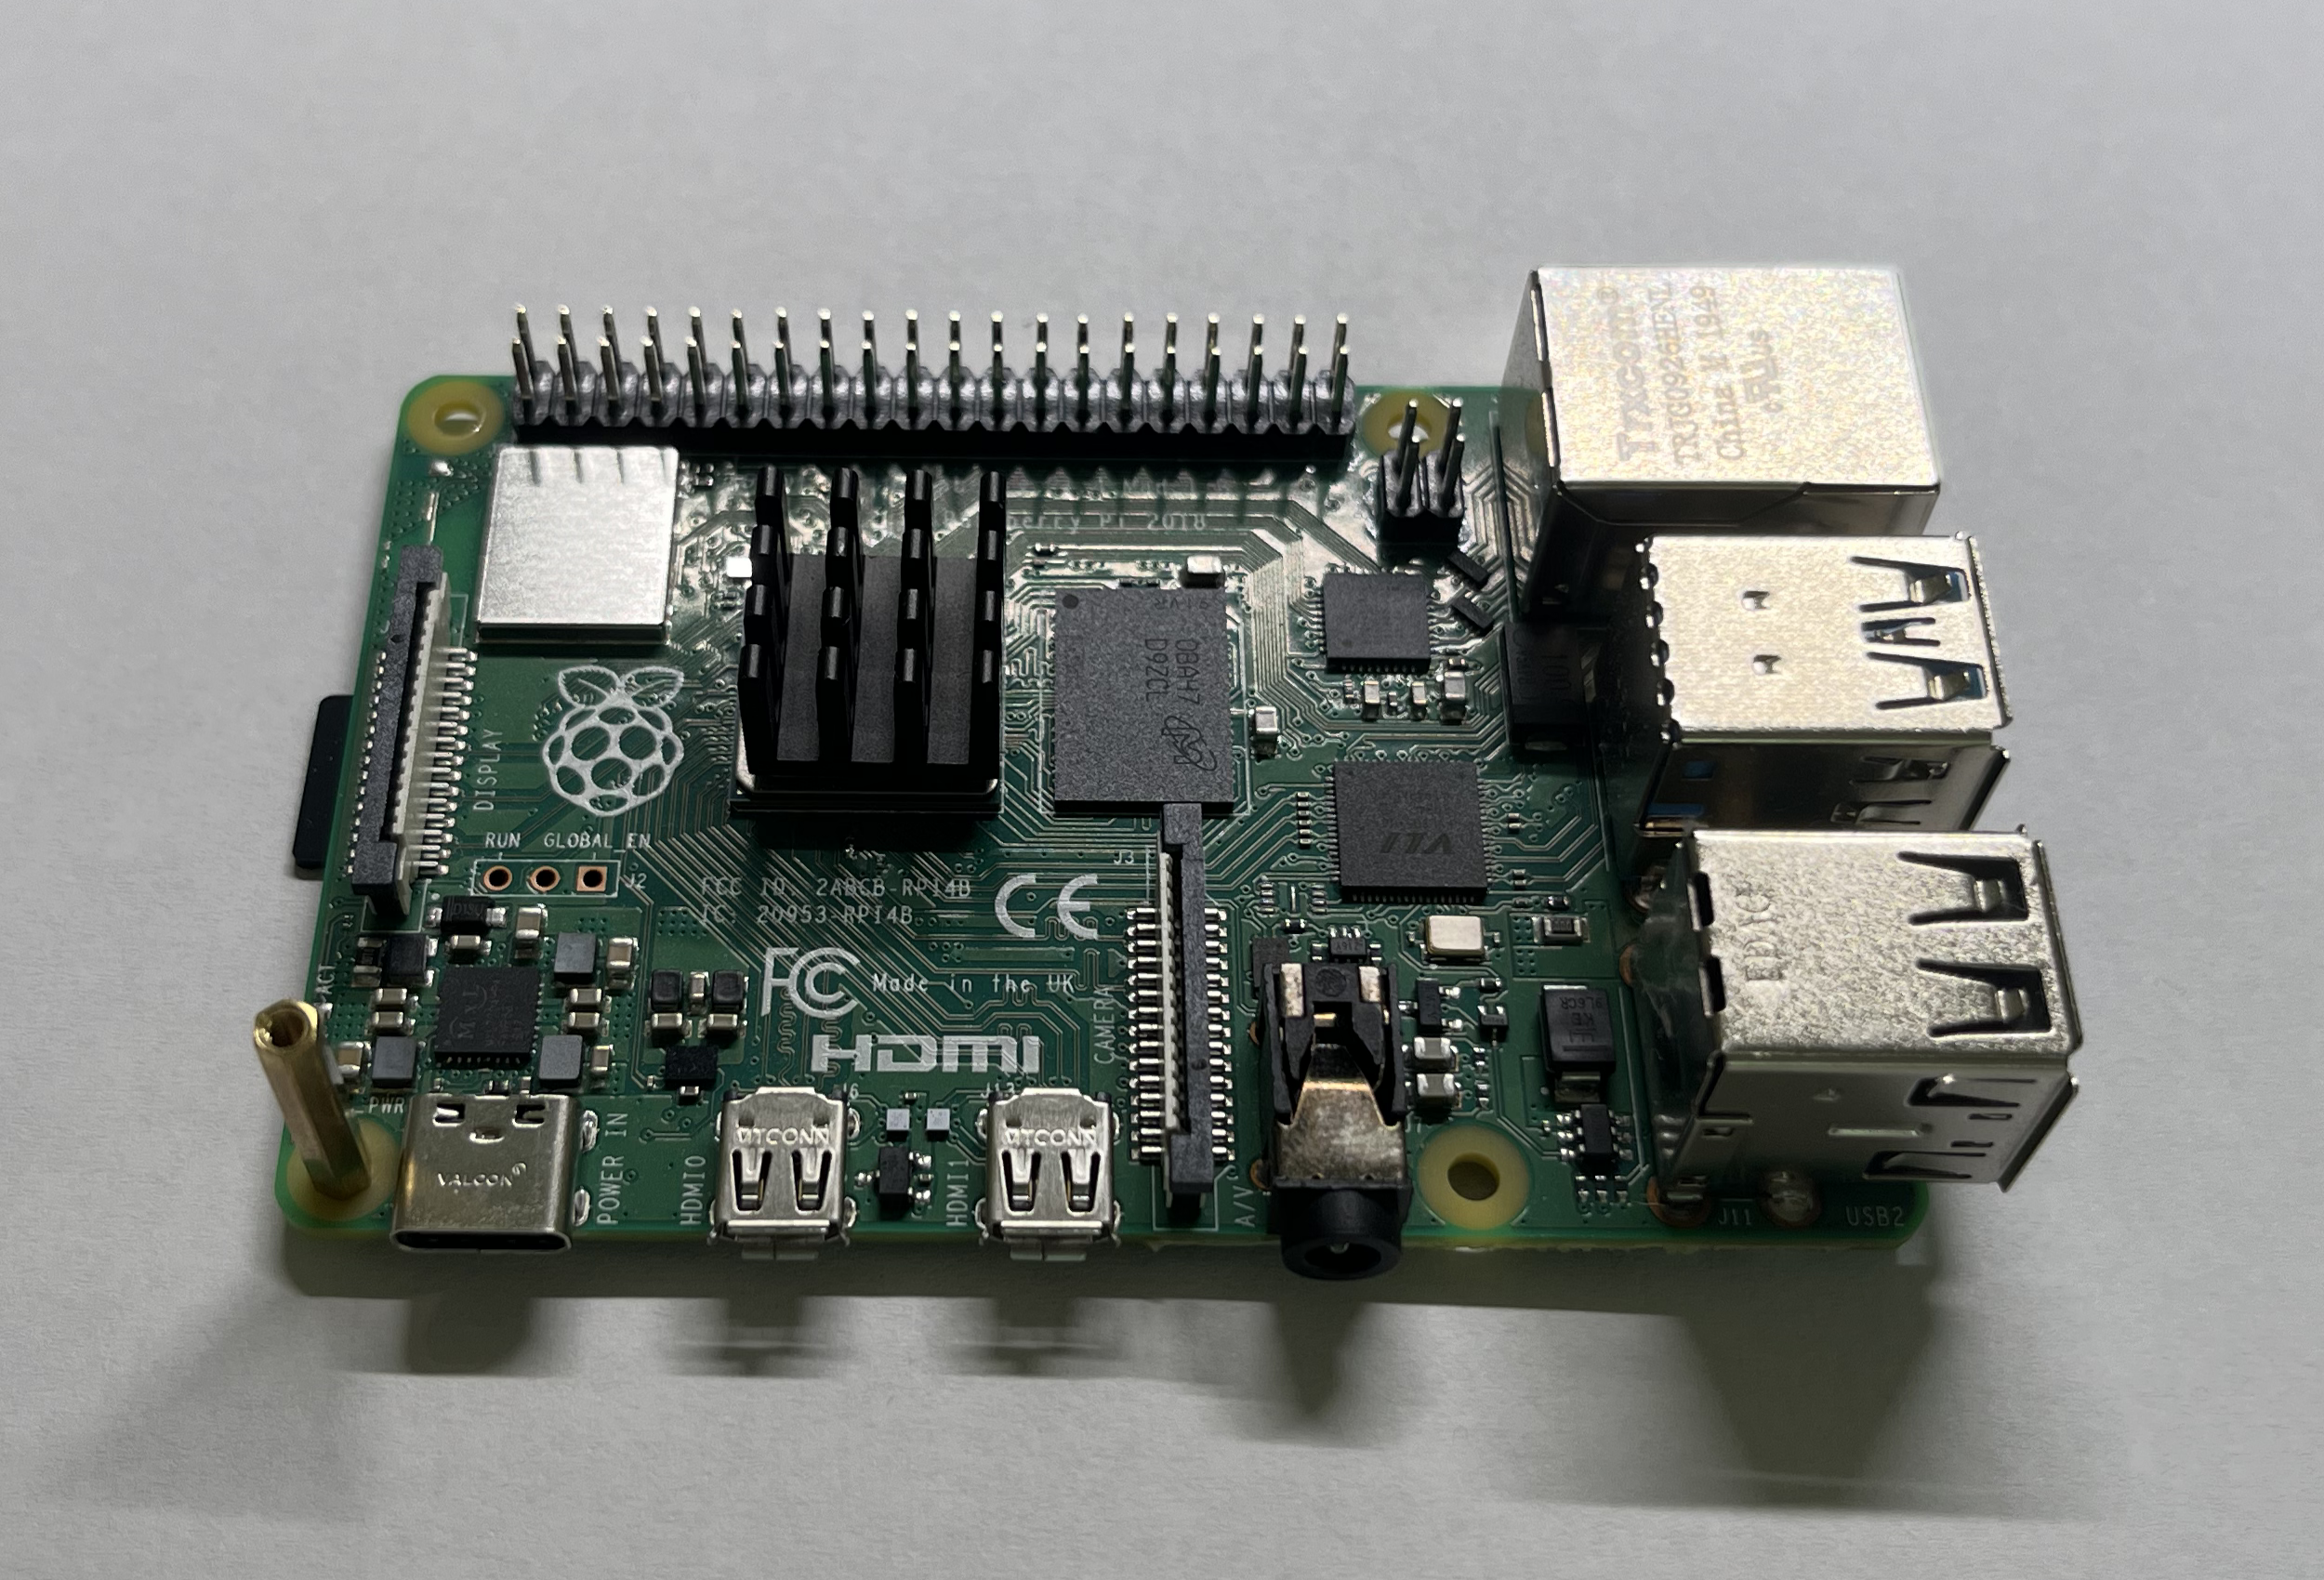
\includegraphics[width=\textwidth]{text/raspberry.png}
        \caption{~Photo of Raspberry Pi 4 B}
        \label{fig:sub2}
    \end{minipage}
    \label{fig:main}
\end{figure}
\chapter{Device Design}
\label{chap:design}


In this chapter, the resulting cloning device, its hardware and software will be designed. The selection of components is based on the Chapter~\ref{chap:analysis}.

\section{Hardware}

After a thorough selection of hardware components, the best combination of the Proxmark 3 Easy reader with a Raspberry Pi 4 B microcomputer was found. These two devices will be connected by a USB-to-micro USB cable, where the male ends can be connected with the shortest possible connection cable to save space in the final device. This cable will provide all communication between the microcomputer and the reader, and will also power the Proxmark 3 Easy via this cable. On the Raspberry Pi itself, a Waveshare 3.5" LCD touchscreen will be connected via pins, which is the size of a microcomputer. The image will be transmitted via the pins and the screen will be powered via this route. An illustration of the component wiring can be seen in the Figure~\ref{fig:devicescheme}. 


\begin{figure}[ht]
  \centering
  \includegraphics[width=6cm]{text/device_scheme.pdf}
  \caption[Illustration of component wiring.]{~Illustration of component wiring.}
  \label{fig:devicescheme}
\end{figure}

To ensure greater battery life and the renewability of the power source, it is best to power the device using a power bank, which will be connected externally to the device using a classic USB-C cable. It is recommended that the power bank supplies the device with 5V/3A~\cite{raspberrydoc}.

This design makes the device compact and easy to use. On the top touch screen, the user controls the device and attaches cloned tags from the bottom of the device. It should be noted that the Proxmark 3 Easy has the LF and HF antenna in different locations, the user must then attach the tag to the specific antenna as needed.

The Proxmark has a button on its longer side that is used to control some of its functions. It is important because card emulation is terminated with this button. It is therefore necessary to make this button accessible to the user.


\section{Software}

This section will justify the selection of the software parts of the project.

\subsection{Operating System}

With the selection of the Raspberry Pi microcomputer, it became clear that Linux would be used as the operating system of the device. It is possible to choose a specific Linux distribution, but for this purpose the official Raspberry Pi OS, which can be obtained for free from the Raspberry~Pi~\cite{raspberrypios} website, will suffice.

The instructions for installing the LCD touch screen drivers recommend the Linux version of bullseye, 32 bit. For the purposes of this device, this version of Linux is suitable.~\cite{waveshare35inch}

The operating system will run in the background of the device, the user will not be able to manipulate the operating system in any way --- and therefore, when Linux starts, the program created will automatically run and take up the entire screen. When the program is finished, the computer itself will shut down. A slight but tolerable drawback is the startup time.

Since the device will be controlled by touch screen, the operating system will have to be adapted to this, and therefore at least make the mouse cursor invisible.

\subsection{Communication With Proxmark}
\label{subsec:communication}

Proxmark 3 Easy is controlled via the commandline client, see Figure~\ref{fig:pm3}. Single commands are sent to the reader to perform operations, such as reading or writing tags. It is also possible to start the client to perform only one specific operation. An output is sent back from Proxmark, which contains various information, such as the success of the operations, or an enumeration of the tag contents. The created program will therefore communicate with Proxmark by starting a process where it sends a specific operation to Proxmark for execution, then parsing the output and passing the necessary feedback to the user. It will also need to ensure that the program checks the availability of Proxmark to avoid errors.

\begin{figure}[ht]
  \centering
  \includegraphics[width=10cm]{text/pm3.png}
  \caption{~Preview of Proxmark commandline client.}
  \label{fig:pm3}
\end{figure}

Some Proxmark operations, such as emulation of some tag types, cannot be terminated by user input in the client, but by pressing a physical button on the Proxmark itself. For this reason, the button will need to be accessible.


\subsection{Programming Language}

The Subsection~\ref{subsec:communication} shows that the program with the graphical environment itself will not actually do any complex calculations, it will only send commands to Proxmark and parse the output. For this reason, the Python programming language is an excellent choice. Man can choose from quite a few graphical libraries to create a graphical interface, and parsing the output is very straightforward.

\subsubsection{Python Graphical User Interface Library}

There are no big demands on the GUI library, from many suitable ones such as PyQt5~\cite{pythonpyqt5}, Kivy~\cite{pythonkivy}, or TKinter~\cite{pythontkinter} the PyQt5 library was chosen, which coincidentally is already part of the Rasperry Pi Os Bullseye 32 bit operating system. This library provides everything needed to create a GUI program.


\subsection{Program}

The program itself must therefore give the user the ability to easily control Proxmark. It must allow the user the following functions:

\begin{itemize}
    \item display basic information about the attached tag,
    \item dumping and storing data of different tag types,
    \item cloning saved dumps into new tags,
    \item manually edit the UIDs of different tag types,
    \item emulate the content of different tag types and
    \item emulate UIDs of different tag types.
\end{itemize}

When it comes to displaying various information about the attached tag, the Proxmark output itself is already clear and needs almost no editing.

Storing tag dump data will force the existence of a repository in Proxmark where the dumps will be stored. The program itself will then need to include an interface where the user can browse these files.

Manual editing of UIDs will require some sort of on-screen keyboard where the user can enter input. There is a solution of a pop-up keyboard, but a more elegant solution is to create a custom keyboard where only the keys that are needed will be present. The UID is simply read in hexadecimal format, so it will be sufficient if the keyboard contains only the characters 0--9 and A--F.

\subsubsection{Architecture}

The PyQt5 library offers a relatively simple way to manage individual screens. The QStackedWidget class will allow you to hold individual widgets\footnote{Widget is the class representing the screen for us at the moment}. Inside the widget, the screen layout can be arranged in a simple way by aligning or applying individual styles. Each screen, i.e. widget, will hold its sub-screens (submenus). This hierarchy allows for easy navigation through the code.

Next, you will need to have a class, let's call it CommandExecutor, which will take care of executing individual operations on the Proxmark.

A class called CommandBuilder will prepare individual commands for the CommandExecutor class to execute, depending on the user's input.

And of course, you will also need to have a class that will process the output received from the Proxmark, and forward the signals back to the user.

For working with files it will be useful to create a class with methods that will take care of this work. 

For easier debugging, it will be smart from the beginning to implement a logging system that will store all logs in a file and that can be looked at and evaluated later.

The process of executing a command --- how the classes will pass information to each other can be seen in Figure~\ref{fig:architecture}.

\begin{figure}[ht]
  \centering
  \includegraphics[width=\textwidth]{text/architecture.pdf}
  \caption{~Information flow between classes.}
  \label{fig:architecture}
\end{figure}


\subsubsection{GUI Design}

First of all, it is important to design how the user interface of the program will look like. Since it will run on a small display with a resolution of only 480 × 320, the GUI must be well laid out and easy to use.

To keep it simple, the best solution will be to create some menus and submenus that the user will navigate back and forth through. This will ensure simplicity of operation on the touchscreen and allow for a relatively small number of buttons in a single menu. This will ensure that everything will always fit on the small screen and there will be no problem with lack of space. In some situations, however, there may be a problem that more content needs to be displayed than can fit on one screen, for example when displaying a list of saved tags. Such a situation can be solved by inserting a scrolling area, where it will be possible to scroll in the user interface.

To get an idea of how such an interface would look like, we can refer to Figure~\ref{fig:wireframe1}, Figure~\ref{fig:wireframe2} and Figure~\ref{fig:wireframe3} containing black and white wireframes.


\begin{figure}[h]
    \centering
    \begin{minipage}[b]{0.315\textwidth}
        \centering
        \includegraphics[width=\textwidth]{text/wireframe1.pdf}
        \caption{~Wireframe 1.}
        \label{fig:wireframe1}
    \end{minipage}
    \hfill
    \begin{minipage}[b]{0.315\textwidth}
        \centering
        \includegraphics[width=\textwidth]{text/wireframe2.pdf}
        \caption{~Wireframe 2.}
        \label{fig:wireframe2}
    \end{minipage}
    \hfill
    \begin{minipage}[b]{0.315\textwidth}
        \centering
        \includegraphics[width=\textwidth]{text/wireframe3.pdf}
        \caption{~Wireframe 3.}
        \label{fig:wireframe3}
    \end{minipage}
\end{figure}


\chapter{Implementation}

This chapter will describe the process of implementing the device --- the commissioning and modification of the computer operating system, the installation of the necessary software and the actual implementation of the program. Any changes to the design of the device will be discussed.

\section{Installing the Operating System}

As mentioned in the design chapter, the appropriate operating system for the Raspberry Pi is Raspberry Pi OS Bullseye 32 bit, partly because of its compatibility with the touchscreen used. The installation is straightforward, using the Raspberry Pi Imager to install the selected system version on the SD card. A Kingston 32 GB SD card was used, although 8 GB would also be sufficient. To get the device working, it is also necessary to provide an internet connection to download the necessary packages, so the device was connected to WiFi. Also, ssh needs to be set up so that the device can be configured remotely when the touchscreen is not yet in use. It should be noted that the system user name must be left \texttt{pi}, otherwise the touchscreen driver installation script does not work correctly. The error is caused by using an absolute path with the user name \texttt{pi} in the installation script, and therefore with a user of a different name the script does not work as it should.   

After successfully uploading the operating system to the SD card, the card was inserted into the device to test its functionality by booting and connecting from a remote computer on the same network.  

\section{Required Packages}

Once the operating system has been successfully commissioned, it is necessary to download the necessary packages to install both the screen driver and the Proxmark software. The following script in Code listing~\ref{code:packages} updates the system and downloads necessary packages.

\begin{lstlisting}[
  caption={~Updating and downloading the necessary packages.},
  label={code:packages},
  language=bash,
  basicstyle=\ttfamily,
  breaklines=true,
  frame=single, 
  keywordstyle=\color{blue},
  commentstyle=\color{green!40!black}, 
  stringstyle=\color{red},
  captionpos=b ]
#! /bin/bash

sudo apt update
sudo apt upgrade
sudo apt install libreadline-dev gcc-arm-none-eabi libssl-dev cmake liblz4-dev libbz2-dev
\end{lstlisting}


\section{Touch Screen Drivers Installation}

After installing the necessary packages, it is necessary to install the driver for the Waveshare LCD 35B-V2 touch screen. This has been performed according to the tutorial in~\cite{waveshare35inch}. Additionally, in Code listing~\ref{code:driver}, the script for installing that driver is provided.

\begin{lstlisting}[
  caption={~Installing the touchscreen driver.},
  label={code:driver},
  language=bash,
  basicstyle=\ttfamily,
  breaklines=true,
  frame=single, 
  keywordstyle=\color{blue},
  commentstyle=\color{green!40!black}, 
  stringstyle=\color{red},
  captionpos=b ]
#! /bin/bash

cd ~
git clone https://github.com/waveshare/LCD-show.git
cd LCD-show/
chmod +x LCD35B-show-V2
./LCD35B-show-V2 # For this specific display, this  LCD35B-show-V2 script must be used
\end{lstlisting}

\section{Proxmark Software Installation}

The Iceman Fork is a very well maintained repository with software for Proxmark devices. This repository on Github~\cite{githubproxmark} will be used for Proxmark software installation.  It contains a client, but also scripts to flash the Proxmark itself.

Using the installation procedure given in~\cite{githubproxmarkdoc}, the software can be installed without any problem. It should be mentioned that before starting the compilation, it is necessary to change the platform in the \texttt{Makefile.platform} configuration file to \texttt{PM3GENERIC}, for which the program will be compiled. It is also necessary to pay attention to the ModemManager, which could damage the device.

\subsection{Flashing Proxmark 3 Easy}

After successful compilation and installation, you can also follow the instructions on Github~\cite{githubproxmarkdoc}. Proxmark 3 Easy can of course also be flashed from a computer other than a Raspberry Pi. 

\section{Operating System Customization}

The following steps are provided to improve the appearance of the software itself, and to create some limitations for users, to have their use of the device limited to the single application:

\begin{itemize}
    \item removing the mouse cursor from the screen,
    \item autostarting the program when the operating system starts,
    \item disabling all unused features such as WiFi or Bluetooth (not done at first for testing purposes).
\end{itemize}

To remove the cursor, the \texttt{/etc/lightdm/lightdm.conf} file needs to be modified, changing \texttt{xserver-command} to \texttt{xserver-command = X -nocursor}. As a result, the cursor is no lonoger visible but the touch screen control works as it should.

Executing the program automatically upon start is done by putting a desktop file in the \texttt{\textasciitilde{}/.config/autostart} folder.


\section{Program Implementation}

This section will explain the principle and description of implementation of the GUI program that controls Proxmark 3 Easy.

\subsection{Architecture}

The implementation followed the design outlined in Chapter~\ref{chap:design}. This means that the \texttt{PyQt5} library allowed for a great layout of individual screens. Thus, each class representing a screen also has a \texttt{QStackWidget} class variable that holds the individual sub-screens.

The program's basic architecture of is depicted in a simplified class diagram in Figure~\ref{fig:classdiagram}. The main class, \texttt{MainWindow}, represents the program window. Then, there are different screens like \texttt{MainScreen}, which contain more screens or other parts of the interface. The implementation also made a great use of class inheritance, where, for example, all screens inherit from one abstract class called \texttt{BaseScreen}. Class inheritance was also used in other cases such as buttons or notification toasts\footnote{A notification toast is a brief, non-interactive alert message that appears temporarily on a mobile device or computer screen, typically in a corner or at the top of the screen.}. This made it easy to create a simple menu in the program. The command execution was implemented as planned in Chapter~\ref{chap:design}.

\begin{figure}[hp]
  \centering
  \includegraphics[width=\textwidth]{text/implementation/uml_class_diagram.pdf}
  \caption{~Simplified class diagram describing the GUI part of the software.}
  \label{fig:classdiagram}
\end{figure}

\subsection{Communication With Proxmark}

The program communicates with Proxmark as follows. The Proxmark client has an option to start itself to execute only single command, which when terminated, will terminate the process itself. An example of running the client this way is shown in Code listing~\ref{code:singlecommand}.

\begin{lstlisting}[
  caption={~Starting Proxmark client to execute given command.},
  label={code:singlecommand},
  language=bash,
  basicstyle=\ttfamily,
  breaklines=true,
  frame=single, 
  keywordstyle=\color{blue},
  commentstyle=\color{green!40!black}, 
  stringstyle=\color{red},
  captionpos=b,
  showstringspaces=false]
pm3 -c 'lf search'
\end{lstlisting}

The \texttt{CommandExecutor} class receives individual commands from the \texttt{CommandBuilder} class. These are then started in the \texttt{CommandExecutor} class as a new process, see Code listing~\ref{code:process}. "\textit{The subprocess module allows you to spawn new processes, connect to their input/output/error pipes, and obtain their return codes.}"~\cite{pythonsubprocess}



\begin{lstlisting}[
  caption={~Starting subprocess in Python.},
  label={code:process},
  language=python,
  basicstyle=\ttfamily,
  breaklines=true,
  frame=single, 
  keywordstyle=\color{blue},
  commentstyle=\color{green!40!black}, 
  stringstyle=\color{red},
  captionpos=b ]
process = subprocess.run(command, shell=True, capture_output=True, text=True)
\end{lstlisting}

Then the output of the executed command is passed to the \texttt{OutputHandler} class, which extracts important information from the output depending on the command, e.g. the success rate of execution or some other information like the UID of the tag. This information is then passed to the UI itself. Before each command is executed, the connection of Proxmark 3 Easy to Raspberry Pi is checked. This is done to determine in case of failure exactly why the command was not executed. A simple activity diagram depicting the process of reading and saving a tag information can be seen in Figure~\ref{fig:activitydiagram}.

\begin{figure}[ht]
  \centering
  \includegraphics[width=\textwidth]{text/implementation/activity_diagram.pdf}
  \caption{~Simplified activity diagram for reading and saving tag information.}
  \label{fig:activitydiagram}
\end{figure}

\subsection{Graphic User Interface}

The creation of the GUI followed the design presented in the Chapter~\ref{chap:design}. The resulting design is therefore very simple and intuitive. An example of it can be seen in Figure~\ref{fig:ui1}, Figure~\ref{fig:ui2} and Figure~\ref{fig:ui3}.

\begin{figure}[h]
    \centering
    \begin{minipage}[b]{0.315\textwidth}
        \centering
        \includegraphics[width=\textwidth]{text/implementation/ui1.png}
        \caption{~Resulting GUI 1.}
        \label{fig:ui1}
    \end{minipage}
    \hfill
    \begin{minipage}[b]{0.315\textwidth}
        \centering
        \includegraphics[width=\textwidth]{text/implementation/ui2.png}
        \caption{~Resulting GUI 2.}
        \label{fig:ui2}
    \end{minipage}
    \hfill
    \begin{minipage}[b]{0.315\textwidth}
        \centering
        \includegraphics[width=\textwidth]{text/implementation/ui3.png}
        \caption{~Resulting GUI 3.}
        \label{fig:ui3}
    \end{minipage}
\end{figure}


\subsubsection{Feedback to the User}
For a better and more intuitive feeling of use, graphical elements had to be implemented to give the user a kind of feedback that conveys information about, for example, whether the entered command was executed correctly or not, or whether an operation is still in progress.

One of these elements was the blocking of buttons that for some reason should not yet be pressable, e.g. when UIDs are not entered when changing UIDs.

For better feedback to the user, notification toasts were used as a method of user notification. The existing \texttt{pyqt-toast} package available here~\cite{toast} was used. The package license is included in the attachment.


\subsection{User Input}

For input purposes, a custom keyboard containing only the characters 0--9 and A--F was created to edit the UID tag. This option was chosen because it is simpler and more practical than a pop-up keyboard that would already be part of the operating system. The main reason was also to limit input, since the user does not need to and should not be able to enter characters other than those listed above anyway. Another reason for using a custom keyboard was also from a visual point of view. A screenshot of the created keyboard can be seen in Figure~\ref{fig:keyboard}.

\begin{figure}[ht]
  \centering
  \includegraphics[width=6cm]{text/implementation/keyboard.png}
  \caption{~Screenshot of the created keyboard.}
  \label{fig:keyboard}
\end{figure}


\subsection{Parsing of the Output}

After each command is executed, its output is processed. Since almost every command has different outputs, it was necessary to test all situations, how each command reacts for example to incorrect input or in what form important information appears in the text. 

This is handled by the aforementioned \texttt{OutputHandler} class. An example of how the handling of the output of one of the commands, specifically the \texttt{hf mf autopwn} command, is handled can be seen in Code Listing A. The outputs of other commands were handled in a similar way --- that is, always looking for a particular string in the output. The extraction of other information, here specifically file names from the output, can also be seen in the sample.

\begin{lstlisting}[
  caption={~Processing output of a command in Python.},
  label={code:processingoutput},
  language=python,
  basicstyle=\ttfamily,
  breaklines=true,
  frame=single, 
  keywordstyle=\color{blue},
  commentstyle=\color{green!40!black}, 
  stringstyle=\color{red},
  captionpos=b,
  showstringspaces=false]
def handle_autopwn_mf_card(self):
        dump_file = self.extract_filename_from_backticks("bytes to binary file")
        keys_file = self.extract_filename_from_backticks("Found keys have been")
        if self.contains_sentence("No tag detected"):
            return constants.NO_CARD_FOUND
        if dump_file is None or keys_file is None:
            return constants.PROBLEM
        self.output = (keys_file, dump_file)
        return constants.OUTPUT_HANDLED
\end{lstlisting}

\chapter{Device Testing}

This chapter describes the process of testing of the functionality of the device. Testing refers to the robustness of the device itself and testing the functionality of cloning and tag emulation which took place in two layers. In the first layer, the capabilities of Proxmark were tested --- how it can read cards, what information it gives out about the card, how it can detect the keys of different types of Mifare Classic tags and what error messages it gives. This layer builds seamlessly on layer two, which has tested the correctness of the program itself, whether it communicates correctly with Proxmark, and whether it can successfully respond to Proxmark's output, either to notifications of successful operations or to error messages. 


\section{User Notes}

This section presents all the findings and shortcomings that emerged from the testing of the resulting device.

\subsection{Battery Life}
After testing the endurance of the device when powered from a 10,000 mAh power bank, it was found that an idle device, i.e. a switched on Raspberry Pi, with the LCD screen and Proxmark connected, lasts up to 8 hours. This result is very encouraging.

\subsection{Boot Time}
It is essential to mention that one problem starts at boot time. Once the device is plugged into the source, it takes at least about 20 seconds for the device to boot and be usable together with the program created. This is one of the impractical things that has resulted from using this device.

\subsection{Touch Screen}

The use of the touch screen has also shown that it has its shortcomings. Its small refresh rate reduces user-friendliness, and some touches are not detected once in a while. However, these shortcomings do not limit the functionality of the device in any way.

\subsection{Graphical User Interface}
After testing the GUI of the created program, many things were tweaked or corrected.

One of the things that had to be solved was the unpredictable freezing screen when executing a command. This was solved by creating a \texttt{Worker} class that inherits from \texttt{QObject}. This Worker then has the task of managing the created thread that executes the command. The actual implementation can be seen in the code. This method fixes the frozen screen.

Further debugging of the program concerned error messages, so that they are displayed at the right time and disappear appropriately, e.g. when the screen changes.

Another thing that was addressed was making user interaction impossible when a command was in progress --- e.g., disabling buttons.


\section{Tested Tags}
\label{sec:testedtags}

For testing purposes, tags of different types were taken, mostly magic tags. Most of the tags were purchased from China, because of their low price and availability --- there are only a few resellers in our country, who increase the price of these tags. Some of the tags for testing were acquired elsewhere. Here is a list of the specific types of tags that were available for testing the resulting device, most of them are at least two of each, to test cloning, and to be safe, as the tag may get damaged:
\begin{itemize}
    \item Low frequency
    \begin{itemize}
        \item EM410x
        \item EM4x05
    \end{itemize}
    \item High frequency
    \begin{itemize}
        \item Mifare Classic magic tags
        \begin{itemize}
            \item Mifare Classic 1k, 4-byte UID, GEN-2
            \item Mifare Classic 1k, 4-byte UID, GEN-1a/GEN-4
            \item Mifare Classic 4k, 7-byte UID, GEN-3
        \end{itemize}
        \item Mifare Classic non-magic tags
        \begin{itemize}
            \item Mifare Classic 1k, 4-byte UID
            \item Mifare Classic 1k, 7-byte UID
        \end{itemize}
        \item Legic Prime
        \item Mifare Ultralight EV1, non-magic tag
        \item Mifare Ultralight EV1, GEN-2 magic tags
        \item Mifare Desfire, generation 1, 2 or 3
    \end{itemize}
\end{itemize}
Some of these named tags are used for some purpose such as building entrances.

\section{Tag Search Testing}

The program has basic tag identification functions. It can list basic tag information such as UID, magic capabilities or chipset type. This output has been filtered from Proxmark to keep it free of irrelevant information and otherwise more or less preserved. Only 2 scenarios were sufficient to test the functionality, namely when the tag is not near the reader at all --- the program identifies no tag found, and the case when the tag is successfully read. These two scenarios were tested for both LF and HF tags separately.

\section{Tags Cloning Testing}
Testing of tag cloning was done separately for each tag type. It should be noted that tag cloning means transferring the data content of one tag to another while preserving the original manufacturer data --- i.e., for example, the tag UID. Changing the UID is tested later in this chapter.

\subsection{Mifare Classic}
\label{subsec:mifareclassiccloning}

Cloning Mifare Classic tags is one of the most complex cloning used in this work, but still quite straightforward. 

First, it was tested if Proxmark could retrieve the keys of all the tested Mifare Classic tags. With only slight difficulties, all keys were obtained --- even the keys of the non-magic tags. Difficulties encountered can only be attributed to the quality of the data transfer between the reader and the tag. Sometimes other tags near the reader interfered with the communication, sometimes it was enough to move the tag to a better position on the HF tag reader.

Testing was carried out on the available Mifare Classic magic tags and the two classic Mifare Classic tags that are used in real-world applications, for example entrance tags. One of the tags is used to enter an unnamed gym. Reading and searching for keys is done a little differently on each tag, depending on which Mifare Classic vulnerability Proxmark is currently exploiting. Most of the keys were read in about 20 seconds, with one exception which was read in about 60 seconds.

With all the keys retrieved, the tag dumps were also saved. In order to write this data to another tag, the keys of the destination tag must also be saved. Only then can the Mifare Classic tag be written.

Writing all sectors to a Mifare Classic 1k tag takes around 15 seconds, while writing to a Mifare Classic 4k tag sometimes takes up to one minute. The process of cloning this type of tag is the most complicated, also because of the duration.

Therefore, when testing Mifare Classic, I did not come into contact with a tag whose keys could not be obtained in this way. In these cases, the resulting device, in its current state, would not be able to clone the Mifare Classic cards. Verification that the write to the target tag was successful was done by comparing the dumpfiles.

\subsubsection{Real-World Example}
The keys of the aforementioned tag used to enter the gym were successfully retrieved by the device and so were the contents of the card. Unfortunately, this card has a 7 byte UID and is of Mifare Classic 1k type and the only available 7 byte magic tag was Mifare Classic 4k type, the other magic tags only had 4 byte UIDs. However, thanks to backwards compatibility, it was possible to copy the contents of the original tag into the first part of the memory and change the UID accordingly. As a result, there was a tag with the same UID and the same data blocks in sectors 0 to 15. After trying to access the gym with the newly cloned tag, it was found that the access was granted and the system therefore did not check the size of the Mifare Classic.

\subsection{Mifare Ultralight}

Unlike the Mifare Classic, the Mifare Ultralight tag is very straightforward to read. When the device is reading the simplest type of Mifare Ultralight, it reads all pages. However, when the type is Mifare Ultralight EV1, the device reads only the unprotected pages, see Chapter~\ref{chap:theory}. This was verified by testing the reading of Ultralight tags. In a moment the card is read, the data dump is ready to move to another tag. Writing to the target tag went always smoothly, the success of the operation was verified by reading the contents of the written tag. 

\subsection{Legic Prime}

Unfortunately, the cloning of the Legic Prime tag has not been tested as it should. Since there was only one tag available, it was only possible to read that tag and write the same tag again. In this respect, it relied on the software in Proxmark, where it was only possible to determine the success rate of writing to that one tag and not to any other.


\section{Tags Emulating Testing}

The testing of tag emulation was of course limited because the number of different readers is limited. The readers that were available were only those that I had already used myself to enter buildings or for identification, and thus no unauthorized access was gained in any case. Additionally, another Proxmark helped with testing the emulation, which always read what the device was emulating. The emulated data could be used to determine the success rate.

\subsection{Two Types of Emulation}
\label{subsec:twotypes}

If the user is unable to get the entire content of the tag, the Proxmark software allows emulation only of the UID (and its associated manufacturer data) of these types of tags:

\begin{itemize}
    \item EM410x,
    \item Mifare Classic,
    \item Mifare DESFire, and
    \item Mifare Ultralight.
\end{itemize}
The device therefore pretends to the reader as the tag type with the set UID. Of course, any additional data in the tag is incorrect and irrelevant.

Of course, many systems require the tag to contain other inaccessible data that is considered secure. In order to emulate these tags, the device must first successfully read the contents of the tag and, in the case of Mifare Classic, its keys. In this paper, the focus is on emulating the data content of these types of tags:

\begin{itemize}
    \item Mifare Classic,
    \item Mifare Ultralight, and
    \item Legic Prime.
\end{itemize}

\subsection{EM410x}

When trying to emulate EM410x tags, there was a problem that the readers could not detect the emulation. A bug in the developed software can be ruled out thanks to the logs generated by the program. It can therefore be attributed to either the Proxmark3 software controlling Proxmark 3 Easy or it may be a hardware problem. A hardware problem is more likely, as after reviewing the Proxmark community posts, people were experiencing a similar problem, and for some the emulation worked without issue~\cite{notworkingemulation}.

After reviewing the emulation and trying to load the emulated tag with a second Proxmark, the problem was confirmed, namely that the Proxmark does not emulate the tag type EM410x at all. If the above reasoning is correct, this could be fixed by replacing the Proxmark 3 Easy with another unit in which the hardware problem does not occur. However, when the Proxmark of the resulting device was replaced with the second one, the emulation was also unsuccessful. Therefore, it is possible that both of the tested Proxmarks have this defect, but another error cannot be ruled out as well.


\subsection{Mifare Classic}
As mentioned in Subsection~\ref{subsec:twotypes}, the Proxmark software supports emulation of either the UID itself or emulation of the entire tag including sectors. For Mifare Classic, Proxmark supports emulation of the UID only for the types Mifare Classic 1k, Mifare Classic 4k. Emulation of only the UID was successful --- the output of the second Proxmark, that read the emulated data can be seen in Figure~\ref{fig:emulateduidclassic}

\begin{figure}[ht]
  \centering
  \includegraphics[width=12cm]{text/testing/classic_4k_uid.png}
  \caption{~Output of the second Proxmark when reading the emulated UID of Mifare Classic 4k.}
  \label{fig:emulateduidclassic}
\end{figure}

Emulation of all sectors of the tag is supported by Proxmark for types

\begin{itemize}
    \item Mifare Classic 1k,
    \item Mifare Classic 4k,
    \item Mifare Classic 2k,
    \item Mifare Classic Mini.
\end{itemize}

For proper emulation it was first necessary to read a Mifare Classic tag and save a dump of its memory. Testing the reading and cracking of Mifare Classic is described in Subsection~\ref{subsec:mifareclassiccloning}. The emulation was tested with another Proxmark that read the emulated tag to verify correctness. A photo of this process can be seen in Figure~\ref{fig:proxmarkemulatingtesting} and a screenshot of how the second Proxmark read the emulated data can be seen in Figure~\ref{fig:emulatedblocksclassic}.

\begin{figure}[ht]
  \centering
  \includegraphics[width=7cm]{text/testing/two_proxmarks.JPEG}
  \caption{~Two Proxmarks on top of each other --- emulation testing.}
  \label{fig:proxmarkemulatingtesting}
\end{figure}

\begin{figure}[ht]
  \centering
  \includegraphics[width=9cm]{text/testing/whole_mf_classic_4k.png}
  \caption{~Reading emulated blocks of Mifare Classic 1k.}
  \label{fig:emulatedblocksclassic}
\end{figure}

Unfortunately, I did not have the opportunity to test the emulation of the Mifare Classic tag in a working system, e.g. the emulation of the tag used to enter the gym, which I managed to clone, see Subsection~\ref{subsec:mifareclassiccloning}.

\subsection{Mifare Ultralight}

Mifare Ultralight tags can be emulated by Proxmark --- pages that have been read. There is again the possibility of emulating just the UID with undefined data pages. Both were tested with a second Proxmark, where a problem was identified. The Proxmark correctly emulated the entered UID of the tag, however, the ATQA and SAK values were wrong. The original Mifare Ultralight tag has ATQA value \texttt{0044} and SAK \texttt{00}. As seen in Figure~\ref{fig:emulatedidultralight}, the device emulated a tag with ATQA value \texttt{0344} and SAK \texttt{00}.

\begin{figure}[ht]
  \centering
  \includegraphics[width=9cm]{text/testing/id_ultralight_wrong _atqa.png}
  \caption{~Wrong ATQA value while emulating Mifare Ultralight.}
  \label{fig:emulatedidultralight}
\end{figure}

After loading a whole Mifare Ultralight tag into emulator's memory, another problem arose. It was not possible to read the blocks of data of the emulated tag. Unfortunately, I did not come into contact with a real-world use of the Mifare Ultralight tag during the testing, so I do not provide a real-world example. It is not a significant drawback that the emulation of Mifare Ultralight does not work as expected, as there was no problem with Mifare Ultralight cloning.

\subsection{Mifare Desfire}
For Mifare DESfire type tags, Proxmark allows emulation of the tag UID only, and this is of course because the card is not known to be attacked and is considered secure~\cite{preucil2023surveying}. 

Testing was therefore conducted again with the second Proxmark as the reader that could read the UID correctly with appropriate ATQA, SAK and ATS values, see Figure~\ref{fig:desfireemulation}.

\begin{figure}[ht]
  \centering
  \includegraphics[width=13cm]{text/testing/des_emulation.png}
  \caption{~Emulated Mifare DESFire, read by second Proxmark.}
  \label{fig:desfireemulation}
\end{figure}

\subsubsection{Real-World Example}
To test the Mifare DESfire tag emulation, I had two tags used to access an unnamed organization and an unnamed school building --- this tag is used, among other things, to pay for lunches in the school cafeteria and to enter the dormitory. 

For the unnamed organization, simply emulating the 7 byte UID DESFire tag was not enough --- access to the building was not granted. Conversely, for the unnamed school's building entrance, emulation of the UID tag alone passed, for the main entrance and for entrances to individual classrooms within the building, even for entry to the dorm areas. Payment using the emulated tag in the student cafeteria was not tested.

For testing, a given 7 byte UID of the school DESFire tag was written to a 7 byte Mifare Classic 4k tag. With this newly created Mifare Classic tag, access was only granted in the school building and not in the dormitory areas. This is because some of the readers are also checking the type of the tag --- ATQA and SAK values, which were in this case different. However, they were correctly emulated by the device before, that explains the granted access to the emulated DESFire tag.

\subsection{Legic Prime}

The Legic Prime tag emulation was tested again using another Proxmark, which successfully read the emulated Legic Prime tag. A photo from the process can be seen in Figure~\ref{fig:legicemulation}. However, the testing was very limited by the number of available Legic Prime tags. 

\begin{figure}[ht]
  \centering
  \includegraphics[width=10cm]{text/testing/emulating_legic.JPEG}
  \caption{~Emulating Legic Prime tag.}
  \label{fig:legicemulation}
\end{figure}


\section{UID Changing Testing}
Generally speaking, changing the UID of magic tags went smoothly, but it always needs to be considered e.g. which generation of magic tag it is, because these tags are controlled by different commands. A couple of times it happened that the tag was broken in response to the wrong command.

\subsection{EM410x}
Exactly with that tag, it depended on the chipset inside. If the tag UID was changed with the T5577 chipset but the encoding for Q5/T5555 was used, the tag was broken. The tag could be fixed by changing the UID and using the correct encoding.

Otherwise, changing the UID of these tags was very straightforward and there were no problems, which is due to the simple tag architecture.

\subsubsection{Real-World Example}
Since there were a lot of EM410x type LF tags available, both the magic ones that can change the UID, but also the ones that are already in use for some operational purposes, such as building entrances or identification in an unnamed canteen, testing the change of the UID was very straightforward and simple. The device was able to change UID of every given magic tag of type EM410x. Thus, the readers in the given buildings read the content of the magic tags without any problem, granting access for those that had the UID of the original tag. 

\subsection{Mifare Classic}
As seen in section~\ref{sec:testedtags}, there were several types of magic Mifare Classic tags available. Each is controlled by different commands and thus there is a distinction between the different types in the device. Therefore, when changing the UID of a magic Mifare Classic tag, it is first necessary to find out what generation it is. This can be easily determined by an HF search, which will give out important information about the tag. Then the appropriate generation needs to be set in the settings. Changing the UID then goes smoothly, during multiple testing of all available tags no problems arose, except when the generation of the magic tag was set incorrectly. Verification of the UID change was done simply by reloading the tag with the device.


\subsection{Mifare Ultralight}
When testing the Mifare Ultralight tag UID change, there was only a minor issue with one of the three tags. The tag had to be positioned perfectly on the reader for the UID change to succeed. The other two tags had no problem with this. After the UID change, the operation was verified by reloading the tag.

\chapter{Related Work}

Several additional steps are needed to improve this prototype device to make it more compact, and more user-friendly.

One of these steps is to incorporate some batteries directly into the device. While a power bank makes the device portable, the same cannot be said for compactness. To this would be added the incorporation of some sort of start button to start the device. 

It is definitely worth thinking about a different and better touch screen, because with the current one there were problems related to the refresh rate or even in the actual detection of the user's touch.

The next step should be to create a device box, for example in a 3D printer. This would increase the shatter resistance of the device, the overall appearance of the device, but also the compactness of the device, where the user would not be afraid to grab the device in one hand.

It would also be beneficial to modify the operating system running on the Raspberry Pi more, mainly to reduce boot time. Another modification could be a modification to the Proxmark3 program itself, where it would be possible to disable the emulation of certain tags with a simple command rather than a button on the Proxmark.

The door is also open for creating support for more tag types that Proxmark3 itself can handle, or will be able to handle in the future.

Finally, it is definitely important to test the device properly with a large number of tag types, with more than I had available, to find as many bugs as possible within the device software.
\chapter{Conclusion}

% Cílem práce bylo sestrojit open-source zařízení, které bude schopné klonovat a emulovat RFID karty a tagy. Součástí práce mělo být navrhnout hardware a software architekturu přenosného zařízení  with respect to modularity and future extensibility za použitití nějakého commercially available microcomputer such as Raspberry Pi. Poté vytvoření programu umožňující klonování a emulaci alespoň 3 různých tagů, s debugováním přímo ve vytvořeném zařízení. S tím spojený i vývoj user interface který bude umožňovat jednoduché ovládání a interakci se zařízením. Poslední část práce měla zahrnovat otestování zařízení s různými typy RFID tagů a karet a vyhodnocení jeho funkčnosti.

% Byl vytvořen návrh prototypu přenosného a rožšířitelného zařízení využitím microcomputer Raspberry Pi a RFID nástroje Proxmark, který umožnujě klonování nebo emulaci množství těch nejznámějších typů RFID karet a tagů, jako je například Mifare Classic, Mifare Ultralight nebo Legic Prime. Byl vyvinut program v jazyce Python s grafickým rozhraním, který dokáže zařízení jednoduše a intuitivně ovládat.

% Vytvořený prototyp zařízení byl pečlivě otestován na zakoupených i již fungujících tagech a kartách. Vyšlo najevo, že testované karty a tagy dokáže bez větších problémů číst, klonovat i emulovat.

% V téhle fázi vývoje je zařízení pro dané typy RFID technologií funkční, avšak pro vylepšení některých vlastností budou zapotřebí další úpravy.

The aim of the work was to build an open-source device that would be able to clone and emulate RFID cards and tags. Part of the work was to design the hardware and software architecture of a portable device with respect to modularity and future extensibility using a commercially available microcomputer such as Raspberry Pi. Then creating a program allowing cloning and emulation of at least 3 different tags, with debugging directly in the created device. Associated with this is the development of a user interface that will allow easy control and interaction with the device. The last part of the work was to involve testing of the device with different types of RFID tags and cards and evaluating its functionality.

A prototype of a portable and scalable device was designed using a Raspberry Pi microcomputer and the RFID tool Proxmark, which allows cloning or emulation of a number of the most well-known RFID card and tag types such as Mifare Classic, Mifare Ultralight or Legic Prime. A Python program has been developed with a graphical interface that can operate the device in a simple and intuitive way.

The prototype device was carefully tested on purchased and existing tags and cards. It turned out that it can read, clone and emulate the tested cards and tags without major problems.

At this stage of development, the device is functional for the given types of RFID technology, but further modifications will be needed to improve some features.

 % include `text.tex' from `text/' subdirectory

\appendix\appendixinit % do not remove these two commands

% \include{text/appendix} % include `appendix.tex' from `text/' subdirectory

\backmatter % do not remove this command

\printbibliography % print out the BibLaTeX-generated bibliography list

\chapter{Attachments}
% Concents of the attachment

	\dirtree{%
		.1 README.md\DTcomment{a brief description of the content of the medium}.
		.1 impl\DTcomment{implemented source codes}.
		.2 README.md\DTcomment{instructions for setting up the program}.
		.2 src\DTcomment{the python source code}.
		.1 text\DTcomment{the text of the thesis}.
		.2 thesis.pdf\DTcomment{text of the thesis in PDF format}.
        .2 thesis\DTcomment{source form of the work in \LaTeX{} format}.
	}
 % include `medium.tex' from `text/' subdirectory

\end{document}
